\documentclass[12pt]{ociamthesis}  % default square logo 
\usepackage[spanish]{babel} 
\usepackage[utf8]{inputenc}
%\documentclass[12pt,beltcrest]{ociamthesis} % use old belt crest logo
%\documentclass[12pt,shieldcrest]{ociamthesis} % use older shield crest logo

%load any additional packages
\usepackage{amssymb}

%input macros (i.e. write your own macros file called mymacros.tex 
%and uncomment the next line)
%\include{mymacros}
\begin{document}

%this baselineskip gives sufficient line spacing for an examiner to easily
%markup the thesis with comments
\baselineskip=18pt plus1pt


%set the number of sectioning levels that get number and appear in the contents
\setcounter{secnumdepth}{3}
\setcounter{tocdepth}{2}


%\maketitle                  % create a title page from the preamble info
\begin{titlepage}
	\begin{center}
		
\includegraphics[width=5cm]{logo2.png}\\
		\vspace{1cm}
		FACULTAD DE INGENIERÍA\\
		INGENIERÍA CIVIL INFORMÁTICA\\
		\vspace{1cm}
		\LARGE{\textbf{Una arquitectura caché para redes ICN basada en comportamiento de usuario} \\}
		\vspace{1cm}
		\small{Tesis para optar al grado de ingeniero civil en informática.}\\
		\vspace{2cm}
		\textbf{Autor:} \\
		Mathias Nicolas Velilla Brandau.\\
		\vspace{1cm}
		\textbf{Profesores guía:} \\
		Carlos Gomez-Pantoja\\
		Miguel Guitierrez\\
		\vspace{1cm}
		Santiago de Chile, Chile.\\
		\vspace{1cm}
		Abril, 2017
	\end{center}
\end{titlepage}


\begin{romanpages}          % start roman page numbering
\tableofcontents            % generate and include a table of contents
\listoffigures              % generate and include a list of figures
\end{romanpages}            % end roman page numbering

\chapter{Introducción}
\section{Motivación}

El nacimiento del Internet en el año 1958 en EEUU a través de ARPA (\textit{Advanced Researchs Proyects Agency}) tuvo como objetivo la comunicación entre diversas universidades y las entidades militares con propósitos investigativos, la invención del telégrafo, el teléfono, la radio y el ordenador sentaron las bases para el desarrollo de esta nueva tecnología, la cual hoy en día ha revolucionado la informática y las comunicaciones como ninguna otra cosa, convirtiéndose en una herramienta de índole mundial, un mecanismo el cual nos permite diseminar información de manera inmediata , generando un medio de colaboración e interacción entre las personas y los ordenadores, desconociendo su ubicación física.\\

Durante los año 2000 - 2008 el uso diario del Internet en las personas americanas se desplazaba entre un 60 y 70 por ciento[Digital Citize], este aumento en el uso de la Internet, conlleva también a un aumento de la información presente en la web, dando como resultado el desarrollo de aplicaciones las cuales deben interactuar con un gran numero de usuarios y analizando una sobresaliente cantidad de información, motivo por el cual Internet impulsado por las demandas de las aplicaciones cada vez más emergentes y las capacidades de las nuevas redes de comunicación, se ha convertido en un mosaico arquitectónico que resulta en una creciente complejidad y vulnerabilidades imprescindibles, entregando como resultado violaciones de capas, proliferación de subcapas, y la erosión del modelo de extremo a extremo, es bajo esta eventualidad que todos los cambios efectuados concluyen en un aumento de la complejidad, lo cual se traduce en una Internet osificada, es por esta razón que los problemas anteriormente señalados no se encuentran directamente relacionados con los protocolos o mecanismo específicos del Internet actual, mas bien son causados esencialmente por la incapacidad de integrar nuevos mecanismos, lo que quiere decir que los problemas son causados por la arquitectura de Internet y podrían ser resueltos con un nuevo diseño de arquitectura de Internet[2].\\

Como una futura propuesta de arquitectura de Internet, ICN (\textit{Information-Centric Networking}) también llamado \textit{Content Centric Networking} (CCN), pretende motivar la transición arquitectónica de la actual arquitectura centrada en el host a centrada en la información para difundir de manera eficiente y flexible la enorme información generada por una variedad de aplicaciones[1], convirtiéndose este en un enfoque que pretende ayudar a desarrollar la infraestructura del Internet y así apoyar de manera directa el acceso a objetos de datos con nombre (NDO), a modo que lo anteriormente señalado es conseguido gracias a la característica clave del paradigma ICN, la presencia de memoria cache dentro de los nodos ICN, en donde cada uno de los contenidos es nombrado única e independientemente desde la ubicación del productor, facilitando el almacenamiento en cache en los nodos intermediarios. Así, por ejemplo, los consumidores solicitaran contenidos enviando el denominado paquete de interés, el cual lleva el nombre del contenido, mientras que el productor o cualquier nodo que mantenga una copia del contenido puede responder a la petición realizada.\\

A su vez, los usuarios ya antes mencionados como consumidores, realizan peticiones en la web, las cuales siguen una conducta dinámica caracterizándose por un elevado sesgo entre los diferentes conjuntos de peticiones, en otras palabras, dentro del universo de peticiones generadas existen conjuntos de peticiones que son regularmente solicitadas por los consumidores en intervalos de tiempos distintos, por lo contrario, otras peticiones escasamente son solicitadas. Dicho lo anterior, también existen situaciones dentro de un intervalo acotado de tiempo, donde surgen explosiva mente peticiones las que se caracterizan por poseer un contenido en común, las cuales nacen por el desarrollo de un evento de interés popular teniendo como resultado un aumento sustancial en la demanda generada a los nodos, teniendo como consecuencia latencia y congestión en las redes.


\section{Desafíos}
%*******************************************************
Los desafíos que se afrontaran para la realización de proyecto de titulo I, son inicialmente el diseño de una nueva arquitectura de memoria caché para los nodos de las redes \textit{ICN} (\textit{Information Centric Network}), considerando el comportamiento de los usuarios por medio del tráfico de red. En segundo lugar, se debe incorporar una estrategia de caché(políticas de admisión, desalojo y reemplazo) y que será implementada en un simulador denominado \textit{ndnSIM} (\textit{Named Data Networking Simulator}), todo esto con el fin de mejorar resultados(Queresultados) en comparación con otras arquitecturas caché que se encuentran por defecto dentro del simulador(LFU, FIFO).\\

\section{Contribución de la tesis}
El aporte entregado por el proyecto de titulo, se puede identificar inicialmente por la creación diseño de una nueva arquitectura de memoria caché para los nodos de las redes \textit{ICN} (\textit{Information Centric Network}), considerando el comportamiento de los usuarios por medio del tráfico de red. En segundo lugar, se debe incorporar una estrategia de caché(políticas de admisión, desalojo y reemplazo) y que será implementada en un simulador denominado \textit{ndnSIM} (\textit{Named Data Networking Simulator}), todo esto con el fin de mejorar resultados de eficiencia de la memoria caché (Hit's, Miss) en comparación con otras arquitecturas caché que se encuentran por defecto dentro del simulador(LFU, FIFO). No obstante, a continuación se detallaran las contribuciones efectuadas por este trabajo:\\
\begin{itemize}
	\item Diseño de una nueva arquitectura cache bajo el paradigma de las redes ICN, que contenga una subdivisión de tres grupos capaces de retener diferentes tipos de peticiones(intereses) de modo que la eficiencia del nodo se vea afectada positivamente. En cuanto a la división de la memoria caché, el primer segmento se encarga del almacenamiento de peticiones del tipo ráfaga, la segunda de guardar las de tipo permanente y para la ultima sección, la recaudación de peticiones de tipo variables.\\
	\item Creación de una topologia de redes ICN, utilizando el simulador ndnSIM, la cual contenga dentro de sus nodos la arquitectura caché anteriormente señalada con la finalidad de inyectar trafico de datos en base al comportamiento usuario para la obtención de resultados empíricos respecto a la nueva arquitectura caché diseñada.\\
\end{itemize}


\section{Estructura de la tesis}
A continuación se realizara una breve reseña de como se estructura el siguiente trabajo:\\

El capitulo 2 abarca la descripción del problema, en el se define el objetivo general, específicos, hipótesis y los alcances que contiene el proyecto de titulo. Incluyendo también la descripción de la metodología de trabajo utilizada para el progreso del trabajo.\\

El capitulo 3 posee el marco teórico, en el cual se definen diferentes conceptos esenciales para el entendimiento del proyecto del titulo. Dicho lo anterior se encuentran los siguiente conceptos: Redes centradas en la información (ICN), ndnSIM, aplicaciones web de gran escala,el cache, estructura y políticas de remplazo del caché existentes y finalizando con el comportamiento del usuario de manera donde se explica la ley de Zipf y se detallan los tipos de peticiones de usuario.\\

En el capítulo 4 se presenta una revisión bibliográfica de los trabajos realizados respecto a las arquitecturas cache y las políticas de cache implementadas en redes ICN, ademas del revisión de trabajos dentro del simulador ndnSIM, todo esto con el fin de diseñar una arquitectura de cache que no exista en la literatura.\\

\chapter{Descripción del problema}

\section{Contextualización}
-¿Que es el cache y para que sirve?
\section{El problema}
\subsection{Declaración del problema}
\subsection{Diagrama de ishikawa}

\section{Objetivos}
\subsection{Objetivo general}
Optimizar la eficiencia del cache en redes \textit{ICN}, por medio del diseño de una arquitectura caché basada en el comportamiento de los usuarios, dentro del simulador \textit{ndnSIM}.

\subsection{Objetivos específicos}
\begin{itemize}
	\item Determinar los componentes estructurales de las redes \textit{ICN}.
	\item Proponer una arquitectura caché para redes \textit{ICN} que considere el comportamiento usuario.
	\item Incorporar una arquitectura cache en el simulador \textit{ndnSIM}
	\item Comparar el rendimiento de la estrategia caché propuesta con estrategias de la literatura
\end{itemize}

\subsection{Alcance de los objetivos}

\chapter{Marco teórico}
\section{Information Centric Network}
Las redes centradas en la información (ICN, por sus siglas en ingles), es una orientación para el desarrollo de una infraestructura de Internet que apoya directamente el acceso a objetos de datos con nombre (NDO, Named Data Object). Los objetos de datos con nombre se desligan de la ubicación, la aplicación, el almacenamiento y los medios de los transporte, dando paso al almacenamiento en cache y un bajo costo y ubicua replicación en la red, esperando como resultado una mayor eficiencia y seguridad, una mayor escabilidad respecto a la demanda de información/ancho de banda y una superior robustez en escenarios de comunicación desafiantes [1].\\

Dicho lo anterior, las redes ICN se componen de dos tipos de paquetes, los paquetes de interés y los paquetes de datos (Figura 3.1), los cuales son enviados por dos tipos de usuarios el primero denominado consumidor, encargado de enviar paquetes de interés y por otra parte un productor, el cual es el encargado de enviar paquetes de datos.\\

	\begin{figure}[h]
		\centering
		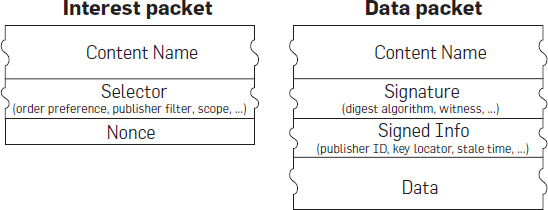
\includegraphics[width=7cm]{Paquetes_CCN.jpg}\\
		\caption{Paquetes CCN}
		\label{fig:mesh1}
	\end{figure} 
Ademas este tipo de redes también cuentan con nodos intermediarios entre los consumidores y los productores, lo que le entrega a la red un aumento en la replicación de información y consigo una mayor resolución de consultas. Los nodos contienen tres estructuras de datos principales(Figura 3.2):\\

\begin{itemize}
	\item\textbf{Forwarding Interest Table (FIB):} El FIB se utiliza para reenviar paquetes de interés hacia fuentes potenciales de datos coincidentes. Es casi idéntico a un IP FIB, excepto que permite una lista de caras salientes en lugar de una sola. Esto refleja el hecho de que CCN no está restringido a reenvío en un árbol de expansión. Permite múltiples fuentes de datos y puede consultarlas todas en paralelo.[3]
	\item \textbf{Almacen de contenido (Content Store (CS):}
	\item \textbf{Pending Interest Table (PIT):} El PIT realiza un seguimiento de los Intereses enviados hacia arriba hacia la(s) fuente(es) de contenido de forma que los Datos devueltos puedan ser enviados aguas abajo a su(s) solicitante(s).[3]
\end{itemize}

	\begin{figure}[h]
		\centering
		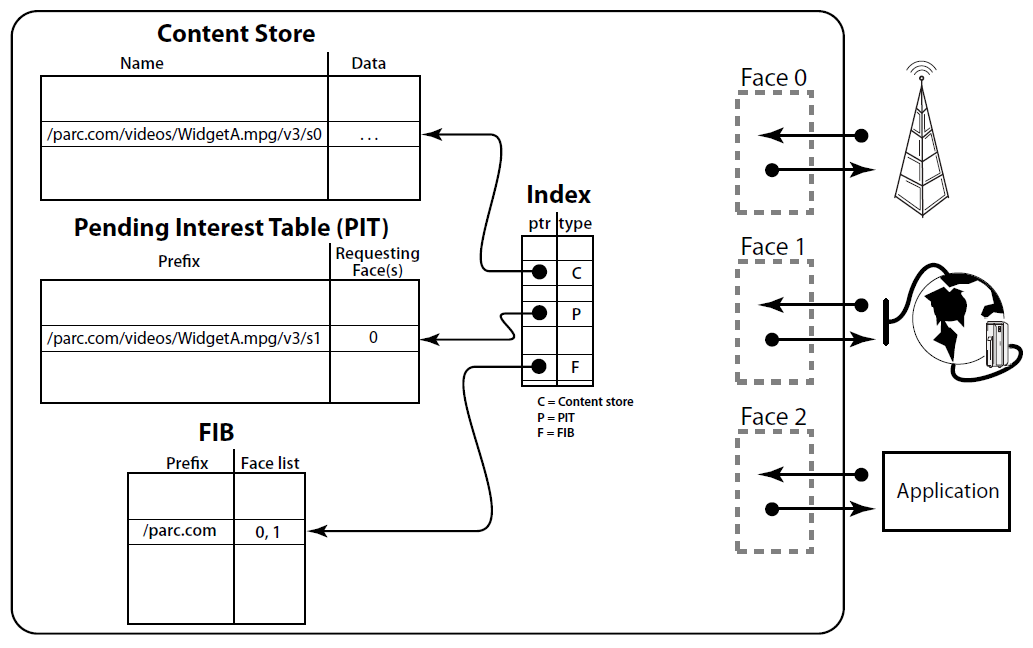
\includegraphics[width=10cm]{Nodo.png}\\
		\caption{Nodo ICN}
		\label{fig:mesh1}
	\end{figure}

\section{Caché}


\section{Comportamiento de usuario}


%*******************************************************
\chapter{Estado del arte}



%*******************************************************
\begin{thebibliography}{a}
	\bibitem{old} \textsc{Kutscher, Dirk, et al.},
	\textit{Information-centric networking (ICN) research challenges.} 2016
	\bibitem{old} \textsc{P. Müller y B. Reuther},
	\textit{Future Internet Architecture–A Service Oriented Approach}, vol. 50, no 6, pp. 383-389, 2009.
	\bibitem{old} \textsc{Jacobson, Van, et al.},
	\textit{"Networking named content."},Proceedings of the 5th international conference on Emerging networking experiments and technologies. ACM, 2009.
\end{thebibliography}

\end{document}

